\chapter{Recunoașterea caracterelor}~\label{chap:recunoastere}
Ultima etapă, aceasta are ca scop identificarea și recunoașterea caracterelor prezente în regiunile selectate în etapa de segmentare.

General vorbind, pentru a atinge acest scop există două variante

\section{Potrivire de șabloane}
Această abordare, cunoscută sub denumirea de template matching, reprezintă metoda clasică de recunoaștere a caracterelor prin compararea directă a pixelilor. Procesul presupune existența unei baze de date cu șabloane (matrice) predefinite pentru fiecare caracter (litere și cifre), care sunt comparate succesiv cu regiunea segmentată până la identificarea celei mai bune potriviri.

Deși este eficientă din punct de vedere computațional datorită simplității algoritmice, această tehnică prezintă limitări severe în scenarii reale. Ea este aplicabilă cu succes doar atunci când caracterele extrase au dimensiuni, fonturi și grosimi constante, fiind extrem de sensibilă la variații geometrice.

Pentru a introduce un grad de robustețe și pentru a atenua sensibilitatea la zgomot sau mici distorsiuni, în locul unei suprapuneri binare perfecte, se utilizează algoritmi bazați pe calcularea distanțelor matematice între vectorii de trăsături: distanța Hamming~\cite{sarfraz2003saudi}, valoarea Jaccard~\cite{lee1994automatic}.

În mod concret,~\cite{sarfraz2003saudi} prezintă un sistem de recunoaștere a caracterelor format din două etape: normalizarea caracterelor și potrivirea șabloanelor. Prima etapă presupune aducerea regiunilor de interes extrase în etapa anterioară la o dimensiune standard de $40\times40$ prin intermediul unei transformări afine care mapează pixelii din imaginea originală la cei ai regiunii determinate anterior.

\begin{figure}[H]
  \centering
  \begin{subfigure}[b]{0.35\linewidth}
    \centering
    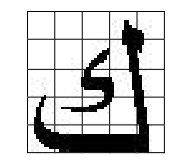
\includegraphics[width=\linewidth]{figures/2003arabia_1.png}
    \caption{}
    \label{fig:2003arabia_a}
  \end{subfigure}
  \hspace{0.05\linewidth}
  \begin{subfigure}[b]{0.35\linewidth}
    \centering
    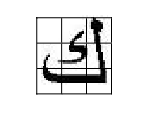
\includegraphics[width=\linewidth]{figures/2003arabia_2.png}
    \caption{}
    \label{fig:2003arabia_b}
  \end{subfigure}
  \caption{ (a) Caracterul original, (b) Caracterul normalizat la o dimensiune standard de $40\times40$~\cite{sarfraz2003saudi}.}
  \label{fig:2003arabia}
\end{figure}

Pentru etapa de potrivire a șabloanelor, precum am menționat anterior, autorii se folosesc de distanța Hamming pentru a determina cel mai apropiat caracter. Formula acestei distanțe este descrisă de Ecuația 4.1.

\begin{equation}
  \begin{split}
    & \sum_{i=1}^{\text{nrows}} \sum_{j=1}^{\text{ncols}} \text{mismatch}_{i,j} \\
    & \text{mismatch}_{i,j} =
      \begin{cases}
        1, & \text{if } \text{original}_{i,j} \neq \text{extracted}_{i,j} \\
        0, & \text{if } \text{original}_{i,j} = \text{extracted}_{i,j}
      \end{cases}
  \end{split}
\end{equation}

\section{Clasificatori statistici}
Această metodă valorifică avansurile recente din domeniul inteligenței artificiale pentru a crea module de recunoaștere a caracterelor (OCR) robuste. Acestea prezintă o rezistența ridicată la variațiile de luminozitate, dimensiuni sau fonturi variate utilizate în creare numerelor de înmatriculare, etc. În literatura de specialitate, cele mai frecvent utilizate modele pentru această etapă a procesării imaginii sunt rețelele neuronale artificiale (ANN) și mașinile pe suport vectorial (SVM), ambele prezentând avantaje și limitări specifice.

S-ar putea spune că există o oarecare similitudine între SVM și ANN deoarece ambele își au rădăcinile în algoritmul perceptronului~\cite{rosenblatt1958perceptron}, însă abordările matematice care precedă acest algoritm diferă fundamental.

\section{Mașini pe suport vectorial}
Algoritmul ce stă la baza mașinilor pe suport vectorial reprezintă o generalizare a algoritmului ”portret generalizat” dezvoltat la începutul anilor 1960~\cite{vapnik1963pattern},~\cite{vapnik1964note}. Fundamentele matematice ale regresiei/ clasficării vectoriale sunt ancorate în învățarea statistică și teoria VC, care oferă o măsură a capacității de învățare a unui algoritm de învățare automată~\cite{vapnik2015uniform}.

Este important de menționat că algoritmul perceptronului funcționează prin actualizarea vectorului de greutăți w pornind de la o valoare inițială arbitrară, de regulă vectorul nul. Acesta este modificat prin adunarea exemplelor pozitive clasificate în mod eronat ca fiind negative, sau prin scăderea exemplelor negative clasificate ca fiind pozitive. Așadar, rezultatul final va fi întotdeauna o combinație liniară a punctelor din setul de antrenament.
\[ \mathbf{w} = \sum_{i=1}^{\ell} \alpha_i y_i \mathbf{x}_i, \]

Unde semnul ecuației este dat de clasificarea $y_i \in \{-1, 1\}$, iar valorile $\alpha_i$ sunt valori pozitive proporționale cu numărul de misclasificări făcute asupra punctului în timpul stagiului de antrenament. Punctele care au cauzat mai puține erori, vor avea un $\alpha_i$ mai mic, iar punctele dificile unul mai mare. Date fiind aceste valori, perceptronul poate fi rescris folosind următoarea formulă:
\[ h(\mathbf{x}) = \operatorname{sgn} \left( \sum_{j=1}^{\ell} \alpha_j y_j \langle \mathbf{x}_j \cdot \mathbf{x} \rangle + b \right) \] numită și forma duală a perceptronului.

Datorită acestei reprezentări duale, este posibilă utilizarea kernel trick-ului care ne permite maparea într-o dimensiune diferită a atributelor primite ca input. O astfel de mapare este benefică deoarece ne permite selectarea și rafinarea atributelor la un nivel mult mai granular. Cu ajutorul kernel trick-ului, algoritmul perceptronului în formă duală nu mai depinde de calcularea explicită a vectorului de greutăți în spațiul trăsăturilor, ci de evaluarea produsului scalar dintre vectorii de intrare mapați
$$ f(\mathbf{x}) = \text{sgn} \left( \sum_{i=1}^{\ell} \alpha_i y_i K(\mathbf{x}_i, \mathbf{x}) + b \right) $$
unde $K(\mathbf{x}_i, \mathbf{x})$ reprezintă funcția kernel, definită ca produsul scalar al funcțiilor de mapare $\phi(\mathbf{x})$ (sau $\theta(\mathbf{x})$).

\section{Teoria VC și clasificatori cu marjă maximală}
Spre deosebire de algoritmul perceptronului, care se oprește în momentul în care identifică un hiperplan care separă corect punctele setului de antrenament, fără a oferi nicio garanție asupra performanței pe date nevăzute, mașinile pe suport vectorial sunt fundamentate teoretic pe principiul minimizării riscului structural derivat din teoria Vapnik-Chervonenkis (VC)~\cite{vapnik2015uniform}.

Conceptul central al acestei teorii îl constituie dimensiunea VC, o măsură a capacității de exprimare a unei familii de funcții de clasificare. În mod formal, dimensiunea VC reprezintă cardinalitatea celui mai mare set de puncte care poate fi etichetat (pulverizat) în toate modurile binare posibile de către funcțiile clasei respective. O dimensiune VC ridicată indică un model cu o capacitate sporită de a se mula pe orice configurație a datelor, dar și un risc proporțional crescut de supra-învățare, deoarece marja garantată între eroarea empirică (pe setul de antrenament) și eroarea reală (așteptată pe distribuția datelor) crește odată cu dimensiunea VC. În consecință, controlul acestei dimensiuni reprezintă o cerință esențială pentru asigurarea capacității de generalizare a modelului.

În cazul particular al hiperplanelor în spațiul $\mathbb{R}^n$, dimensiunea VC este, în general, $n+1$. Totuși, dacă restrângem familia clasificatorilor la submulțimea hiperplanelor care separă datele cu o marjă $\gamma$ și presupunem că punctele de antrenament sunt incluse într-o sferă de rază $R$, atunci dimensiunea VC efectivă a clasei rezultate este mărginită superior de raportul $R^2/\gamma^2$~\cite{vapnik2015uniform},~\cite{svmIntroduction}. Această observație fundamentală oferă justificarea teoretică pentru abordarea adoptată de SVM: prin maximizarea marjei $\gamma$, se reduce implicit dimensiunea VC a familiei de funcții utilizate, ceea ce conduce la limite superioare mai stricte asupra erorii de generalizare, independent de dimensionalitatea spațiului trăsăturilor.

Formal, problema clasificatorului cu marjă maximală se reduce la rezolvarea problemei de optimizare convexă:
\[
\min_{\mathbf{w}, b} \frac{1}{2} \|\mathbf{w}\|^2 \quad \text{cu restricția} \quad y_i(\mathbf{w}^\top \mathbf{x}_i + b) \geq 1, \quad i = 1, \dots, \ell,
\]
unde minimizarea normei $\|\mathbf{w}\|$ este echivalentă cu maximizarea marjei $\gamma = 1/\|\mathbf{w}\|$. Această proprietate este deosebit de relevantă în contextul recunoașterii caracterelor de pe plăcuțele de înmatriculare, deoarece spațiile de trăsături utilizate (vectori obținuți prin caracteristici HOG, momente Zernike sau pixeli normalizați) sunt frecvent înalt dimensionale, iar capacitatea unui clasificator de a evita supra-învățarea într-un astfel de regim este critică.

Pentru a permite tratarea seturilor de date care nu sunt liniar separabile, formularea originală a fost extinsă prin introducerea variabilelor de relaxare $\xi_i$ și a parametrului de penalizare $C$~\cite{cortes1995support}, conducând la formularea cu marjă moale:
\[
\min_{\mathbf{w}, b, \xi} \frac{1}{2} \|\mathbf{w}\|^2 + C \sum_{i=1}^{\ell} \xi_i \quad \text{cu restricția} \quad y_i(\mathbf{w}^\top \mathbf{x}_i + b) \geq 1 - \xi_i, \quad \xi_i \geq 0.
\]
Parametrul $C$ controlează raportul dintre maximizarea marjei și tolerarea erorilor de clasificare, permițând astfel un compromis explicit între capacitatea modelului și riscul empiric. Combinat cu utilizarea funcțiilor kernel introduse prin~\cite{boser1992training}, acest cadru permite construirea unor clasificatori cu putere de discriminare ridicată, păstrând în același timp un control formal asupra capacității de generalizare.

\section{Rețele neuronale artificiale}
Rețelele neuronale artificiale (ANN) reprezintă cea de-a doua direcție majoră în recunoașterea caracterelor din cadrul plăcuțelor de înmatriculare. Spre deosebire de SVM, care își are fundamentul în teoria învățării statistice, ANN-urile sunt inspirate dintr-un model simplificat al activității neuronilor biologici și se bazează pe compunerea ierarhică a unităților elementare derivate din perceptronul lui Rosenblatt~\cite{rosenblatt1958perceptron}.

Perceptronul multistrat (MLP), constă într-un strat de intrare, unul sau mai multe straturi ascunse și un strat de ieșire. Fiecare neuron $j$ dintr-un strat efectuează o transformare afină asupra activărilor stratului precedent, urmată de aplicarea unei funcții de activare neliniare $\sigma$:
\[
a_j = \sigma\left( \sum_{i} w_{ji} x_i + b_j \right).
\]
Compoziția acestor transformări permite rețelei să construiască, în mod implicit, reprezentări ale datelor de complexitate crescândă. Justificarea teoretică pentru această abordare este oferită de teorema aproximării universale, care stabilește că o rețea cu un singur strat ascuns și un număr suficient de neuroni poate aproxima, cu precizie arbitrară, orice funcție continuă definită pe un domeniu compact~\cite{hornik1989multilayer}.

Antrenarea ANN-urilor este realizată prin algoritmul de retropropagare a erorii~\cite{rumelhart1986learning}, urmat de o actualizare iterativă a acestora prin metode bazate pe coborârea gradientului. În contextul recunoașterii caracterelor de pe plăcuțele de înmatriculare, intrarea este, în mod tipic, o imagine segmentată corespunzătoare unui singur caracter, normalizată la o rezoluție fixă, iar ieșirea reprezintă o distribuție de probabilitate peste setul de clase posibile (literele alfabetului și cifrele 0--9), obținută prin aplicarea funcției softmax.

Comparativ cu SVM, ANN-urile prezintă avantajul de a învăța automat reprezentări intermediare ale datelor, fără a necesita o etapă explicită de inginerie a trăsăturilor. Acest fapt este deosebit de util în prezența variațiilor de font, grosime a caracterelor sau ușoare deformări geometrice. Pe de altă parte, antrenarea ANN-urilor necesită seturi de date considerabil mai voluminoase, este sensibilă la inițializarea parametrilor și nu beneficiază de garanții de generalizare la fel de stricte precum cele derivate din teoria VC pentru SVM-urile cu marjă maximală.

